\documentclass{report}

\usepackage{subcaption} % package for subfigures
\usepackage{hyperref}  % package for linking figures etc
\usepackage{enumitem}  % package for description with bullets
\usepackage{graphicx}  % package for importing images
\usepackage{mathtools} % package for math equation
\usepackage{mathrsfs}  % package for math font
\usepackage{indentfirst} % package for getting ident after section or paragraph
\usepackage[export]{adjustbox}
% \usepackage{amsmath}

% \usepackage{array}   % for tables
\usepackage{tabu}   % for tables 
\setlength{\parindent}{2em} % how much indent to use when we start a paragraph

\graphicspath{ {./theory/figures/} }       % path for images

\begin{document}

\chapter{Tube Proposal Network}

One of the basic elements of ActionNet is \textbf{Tube Proposal Network}(TPN). The main purpose of this network is to propose
\textbf{Tube of Interest}(TOIs). These tubes are likely to contain an known action and are consisted of some 2D boxes
(1 for each frame). TPN is inspired from RPN introduced by FasterRCNN\cite{Ren:2015:FRT:2969239.2969250}, but instead of images, TPN
is used in videos as show in \cite{DBLP:journals/corr/HouCS17}. In full correspondence with RPN, the structure
of TPN is similar to RPN. The only difference, is that TPN uses 3D Convolutional Layers and 3D anchors instead of 2D. \par
We designed 2 main structures for TPN. Each approach has a different definition of the used 3D anchors.
The rest structure of the TPN is mainly the same with some little differences in the regression layer. \par
Before describing TPN, we present the preprocess procedure which is the same for both approaches.

\section{Steps before TPN}

\subsection{Preparing data}

Our architecture gets as input a sequnece of frames which has a fixed size in widht, height and duration. However, each video has different resolution. That's creates the
need to resize each frame before. As mentioned in previous chapter, the first element of our network is a 3D RenNet taken from \cite{hara3dcnns}. This network is designed to
get images with dimensions (112,112). As a result, we resize each frame from datasets' videos into (112,112) frames. In order to keep aspect ratio, we pad each frame either
left and right, either above and bellow depending which dimension is bigger. In figure  \ref{fig:Preprocess_example} we can see the original frame and the resize and padded one.
In full correspondance, we resize the groundtruth bounding boxes for each frame (figure \ref{fig:original_image_rois} and \ref{fig:trans_image_rois} show that).

\begin{figure}[h]
  \centering
  \begin{subfigure}{0.35\textwidth}
    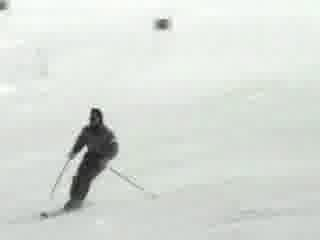
\includegraphics[width=\textwidth]{./figures/original_image.jpg}
    \caption{}
    \label{fig:original_image}
  \end{subfigure}
  \hfill
  \begin{subfigure}{0.35\textwidth}
    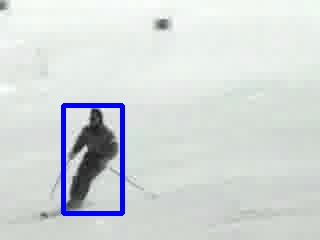
\includegraphics[width=\textwidth]{./figures/original_image_rois.jpg}
    \caption{}
    \label{fig:original_image_rois}
  \end{subfigure}
  \hfill
  \begin{subfigure}{0.35\textwidth}
    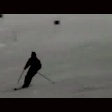
\includegraphics[width=\textwidth]{./figures/transformed_image.jpg}
    \caption{}
    \label{fig:trans_image}
  \end{subfigure}
  \hfill
  \begin{subfigure}{0.35\textwidth}
    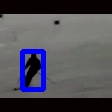
\includegraphics[width=\textwidth]{./figures/transformed_image_rois.jpg}
    \caption{}
    \label{fig:trans_image_rois}
  \end{subfigure}

  \caption{ At (a), (b) frame is its original size and at (c), (d) same frame after preprocessing part}
  \label{fig:Preprocess_example}
\end{figure}


\subsection{3D ResNet}
Before using Tube Proposal Network, we spatio-temporal features from the video. In order to do so, we extract the 3 first Layers of a
pretrained 3D ResNet. It is pretrained in Kinetics dataset \cite{DBLP:journals/corr/KayCSZHVVGBNSZ17} for sample duration = 16 and
sample size = (112,122). \par
This network normally is used for classifying the whole video, so some of its layers use temporal stride = 2.
We set their temporal stride equal to 1 because we don't want to miss any temporal information during the process.
So, the output of the third layer is a feature maps with dimesions (256,16,7,7). We feed this feature map to TPN, which is described
in following sections.

\section{ 3D anchors as 6-dim vector}
\subsection{First Description}
We started desinging our TPN inspired by \cite{DBLP:journals/corr/HouCS17}. We consider each anchor as a 3D bounding box written as
$(x_1, y_1, t_1, x_2, y_2, t_2)$ where $x_1, y_1, t_1$
are the upper front left coordinates of the 3D and $x_2, y_2, t_2$ are the lower back left as shown in figure \ref{fig:anchor_6d}.
\begin{figure}[h]
  \centering
  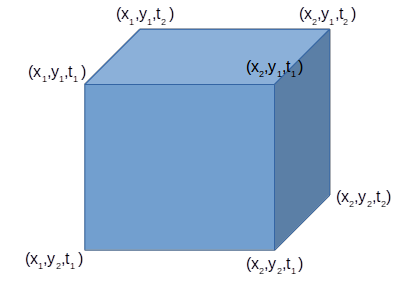
\includegraphics[scale=0.5]{anchor_6d}
  \caption{An example of the anchor $(x_1,y_1,t_1,x_2,y_2,t_2)$}
  \label{fig:anchor_6d}
\end{figure}

The main advantage of this approach is that except from x-y dims, dimension of time is mutable. As a result, the proposed TOIs have
no fixed time duration. This will help us deal with untrimmed videos, because proposed TOIs would exclude background frames.
For this approach, we use \textbf{n=4k=60} anchors for each pixel in the feature map of TPN. We have k anchors for each sample
duration( 5 scales of 1, 2, 4, 8, 16, 3 aspect ratios of 1:1, 1:2, 2:1 and 4 durations of 16,12,8,4 frames).
In \cite{'DBLP:journals/corr/HouCS1},  network's anchors are defined according to the dataset most common anchors. This, however,
creates the need to redesign the network for each dataset. We use the same anchors for both datasets, trying to generalize our
approach.
So the structure of TPN is:
\begin{itemize}
\item 1 3D Convolutional Layer
\item 1 classification layer outputs \textit{2n scores} whether there is an action or not for \textit{n tubes}.
\item 1 regression layer outputs \textit{6n coordinates} ($x_1,y_1,t_1,x_2,y_2,t_2$) for \textit{n tubes}.
\end{itemize}

which is shown in figure \ref{fig:tpn_1_1}
\begin{figure}[h]

  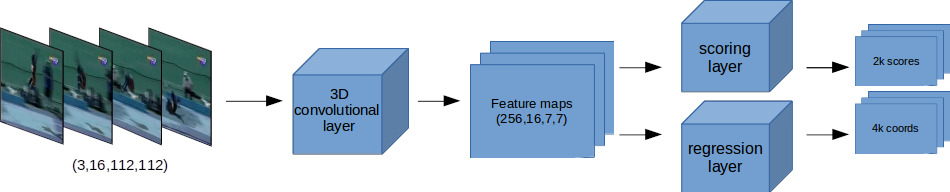
\includegraphics[width=1.\textwidth]{tpn_1_1}
  \caption{Structure of TPN}
  \label{fig:tpn_1_1}
\end{figure}

% \subsection{Preparing Data for training}


\subsection{Training}
As mentioned before, TPN extracts TOIs as 6-dim vectors. For that reason, we modify out groundtruth ROIs to groundtruth Tubes.
We take for granted that the actor cannot move a lot during 16 frames, so that's why we use this kind of tubes. As shown 
in figure \ref{fig:gt_tubes_and_rois}, these tubes are 3D boxes which include all the groundtruth rois, which are different
for each frame.

\begin{figure}[h]
  \centering
  \begin{subfigure}{0.15\textwidth}
    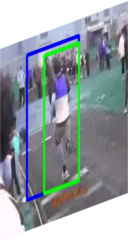
\includegraphics[width=\textwidth]{output/img_0.jpg}
  \end{subfigure}
  \begin{subfigure}{0.15\textwidth}
    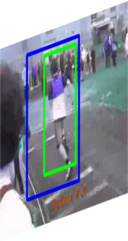
\includegraphics[width=\textwidth]{output/img_3.jpg}
  \end{subfigure}
  \begin{subfigure}{0.15\textwidth}
    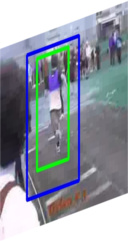
\includegraphics[width=\textwidth]{output/img_5.jpg}
  \end{subfigure}
  \begin{subfigure}{0.15\textwidth}
    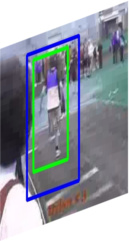
\includegraphics[width=\textwidth]{output/img_7.jpg}
  \end{subfigure}
  \begin{subfigure}{0.15\textwidth}
    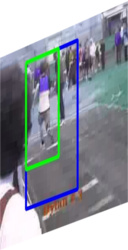
\includegraphics[width=\textwidth]{output/img_11.jpg}
  \end{subfigure}
  \begin{subfigure}{0.15\textwidth}
    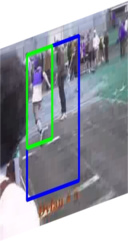
\includegraphics[width=\textwidth]{output/img_15.jpg}
  \end{subfigure}
  \caption{Groundtruth tube is coloured with blue and groundtruth rois with colour green}
  \label{fig:gt_tubes_and_rois}
\end{figure}

For training procedure, for each video, we randomly select a part of it which has duration 16 frames. For each video, we train TPN in
order to score all the anchors using IoU criterion (which is explained in next paragraph) and we use Cross Entropy Loss as a loss function.
For regression, we use smooth-L1 loss. For regression targets, we use the same implementation as Faster R-CNN does, but for 3 domains again.
So we have:
\[ \begin{matrix}
    t_x = (x-x_a)/w_a, & t_y = (y-y_a)/h_a, & t_z= (z-z_a)/d_a, \\
    t_w= log(w/w_a), & t_h= log(h/h_a), & t_d = log(d/d_a), \\
    t^*_x = (x^* - x_a)/w_a, & t^*_y = (y^* - y_a)/h_a, & t^*_z = (z^* - z_a)/d_a, \\
    t^*_w = log(w^* /w_a), & t^*_h = log(h^*/h_a), & t^*_d = log(d^*/d_a),
    % t∗x= (x∗−xa)/wa,  t∗y= (y∗−ya)/ha,t∗w= log(w∗/wa),  t∗h= log(h∗/ha)
  \end{matrix}
\]
where \textit{x, y, z, w, h, d} denote the 3D box's center coordinates and its widht, height and duration. Variables $x, x_a, \text{ and } x^*$
are for the predicted box, anchor box, and groundthruth box respectively (likewise for \textit{y, z, w, h, d}). \par

\paragraph{Modified Intersection over Union(mIoU)}
During training, we get numerous anchors. We have to classify them as foreground anchors or
background anchors. Foreground anchors are those which contain some action. We need a criterion
for evaluating them if we know the groundtruth tubes. We can see an extend of Intersection over Union
criterion, which is used in Object Detection algorithms. So, we will consider as foreground those which
have Intersection Over Union $\ge$ 0.5 . \\
One first approach would be to consider instead of areas, the volume of 2 candidate tubes. So IoU would be:
\[ IoU = \frac{\text{ Volume of Overlap} }{\text{Volume of Union}} \]
Intuitively, the above criterion is good for evaluating 2 tubes if they overlap but it has one big drawback:
it considers x-y dimesions to have same importance with time dimension, which we do not desire. That's becase
firstly we care to be accurate in time dimension, and then we can fix x-y domain.
As a result, we change the way we calculate the Intesection Over Union. We calculate seperately
the IoU in x-y domain (IoU-xy) and in t-domain (IoU-t). Finally, we multiply them in order to get the final IoU.
So the formula for 2 tubes ($x_1, y_1, t_1, x_2, y_2, t_2$) and ($x'_1, y'_1, t'_1, x'_2, y'_2, t'_2$) is:
\[ IoU_{xy} = \frac{ \text{Area of Overlap in x-y}} { \text{Area of Union in x-y}} \]
\[ IoU_t = \frac { max(t_1, t'_1) - min(t_2, t'_2)} {min(t_1,t'_1) - max(t_2,t'_2)} \]
\[ IoU = IoU_{xy} \cdot  IoU_t \]
The above criterion help us balance the impact of time domain in IoU. For example, let us consider 2 anchors:
a = (22, 41, 1, 34, 70, 5) and b = (20, 45, 2, 32, 72, 5). These 2 anchors in x-y domain have IoU score equal to 0.61.
But they are not exactly overlaped in time dim. Using the first approach we get 0.5057 IoU score and using the
second approach we get 0.4889. So, the second criterion would reject this anchor, because there is a difference in time
duration. 
% On top of that, we can add a $\lambda$ factor in order to balance better the ratio between time and x-y domains. So this
% formula is written as:
% \[ IoU = \lambda \cdot IoU_{xy} \cdot  IoU_t \]


\par

% \begin{itemize}
% \item 1 3D Convolutional Layer
% \item 2 classification layers
%   \begin{itemize}
%   \item 1 classification layer outputs \textit{2n scores} whether there is an action or not for \textit{n tubes}.
%   \item 1 classification layer outputs \textit{2k scores} whether there is an action or not for \textit{k tubes}.
%   \end{itemize}
% \item 2 regression layers
%   \begin{itemize}
%   \item 1 regression layer outputs \textit{6n coordinates} ($x_1,y_1,t_1,x_2,y_2,t_2$) for \textit{n tubes}.
%   \item 1 regression layer outputs \textit{6k coordinates} ($x_1,y_1,t_1,x_2,y_2,t_2$) for \textit{k tubes}.
%   \end{itemize}
% \end{itemize}

%% TODO add picture of structure

\subsection{Adding regressor}
The output of TPN is $\alpha$-highest scoring anchors moved according to their regression prediction. After that, we have to translate the anchor into tubes.
In order to do so, we add a regressor system which gets as input TOIs' feature maps and returns a sequence of 2D boxes, each for every frame.
The only problem is that the regressor needs a fixed input size of featuremaps. This problem is already solven by R-CNNs which use roi pooling and roi align
in order to get fixed size feature maps from ROIs with changing sizes. In our situation, we extend roi align operation, presented by Mask R-CNN, and we
call it \textbf{3D Roi Align}.

\paragraph{3D Roi Align}
3D Roi align is a modification of roi align presented by Mask R-CNN\cite{DBLP:journals/corr/HeGDG17}. The main difference between those two is that Mask R-CNN's roi align uses
bilinear interpolation for extracting ROI's features and ours 3D roi align uses trilinear interpolation for the same reason. Again, the 3rd dimension is
time.
So, we have as input a feature map extracted from ResNet34 with dimensions (64,16,28,28) and a tensor containing the proposed TOIs.
For each TOI, we get as output a feature map with size (64, 16, 7, 7). \par
On top of that, for each proposed TOI we give its feature map as input to a regressor. This regressor, returns 16 $\cdot$ 4 predicted translations, 4 for each frame.
We keep only the predicted translations, for the frames that are $\ge t_1$ and $< t_2$. 
\begin{figure}[h]
  \centering
  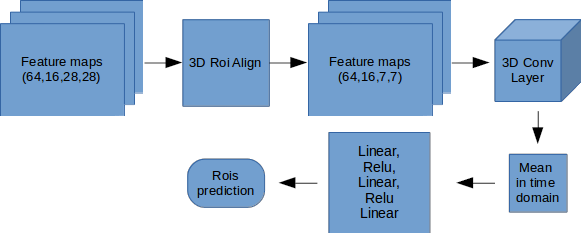
\includegraphics[scale=0.5]{regressor_1_3d}
  \caption{Structure of Regressor}
  \label{fig:regressor_3d}
\end{figure}

Finally, for the frames, contained by the anchors, we set a 2D box ($x_1,y_1,x_2,y_2$) where $x_1, y_1, x_2, y_2$ are the reggressed values from the anchor,
and the frames which are not contained, we set a zero-ed 2D box. The previous regressor is also trainable. It is consisted of 1 2D convolutional layer followed by a
Relu function and another Linear Layer as shown in figure \ref{fig:regressor_3d}. After getting proposed TOIs from TPN, we pick, randomly, 16 tubes which will be input in the regressor.
Finally, we find the traslation for each rois and, again, we use smooth-L1 loss for loss function.\par

\subsection{Validation}

Validation procedure is a bit similar to training procedure.
We randomly select 16 frames from a validation video and we examine if there is at least 1 proposed TOI
which overlaps $\ge$ 0.5 with the groundtruth tubes. If there is, we consider this tube as True Positive (TP) else as False Negative (FN).

After we run one epochfor the whole validation dataset we calculate the \textbf{recall} metric which is:
\[ recall = \frac{\text{TP}} {\textbf{TP + FN}} \]

In order to count overlaps we use 2 kinds of Iou metrics.
\begin{enumerate}
\item 3D IoU which was mentioned before, which counts tubes' Volumes' Intersection of Union (without the modification we made during training).
\item the mean ROIs'  IoU for each frame.
\end{enumerate}
Respectively, we calculate 2 kinds of recall. The first one tells as how good were our proposed TOIs. The second one tells us how many tubes,
we managed to detect during our proposals. \textbf{We count another one recall, which tells us how many from the good Proposed TOIs
   managed to correspond to an actual tube. In other words, this metric shows us the performance of the regressor.}

  
\paragraph{}
In order to get good proposal, after TPN we use Non-Maximum Suppresion (NMS) algorith. This algoriths removes at the proposed TOIs which have overlap > 0.7 with the
high-scoring proposed TOIs. As we can see in table {}, we get better recall scores when using NMS algorithm.

\subsection{Improving TPN score}
After first test, we came with the idea that in a video lasting 16 frames, in time domain, all kind of actions can be seperated in the following categories:
\begin{enumerate}
\item Action starts in the n-th  frame and finishes after the 16th frame of the sampled video.
\item Action has already begun before the 1st frame of the video and ends in the n-th frame.
\item Action has already begun before the 1st frame of the video and finishes after the 16th video frame.
\item Action starts and ends in that 16 frames of the video.
\end{enumerate}

On top of that, we noticed that most of actions, in our datasets, last more that 16 frame. So, we added 1 scoring layer and 1 reggression layer as shown in 
figure \ref{fig:tpn_1_2}. These two layers have anchors with fixed time duration. Their purpose is to be trained only in x-y domain, keeping time duration
steady. 
\begin{figure}[h]
  \centering
  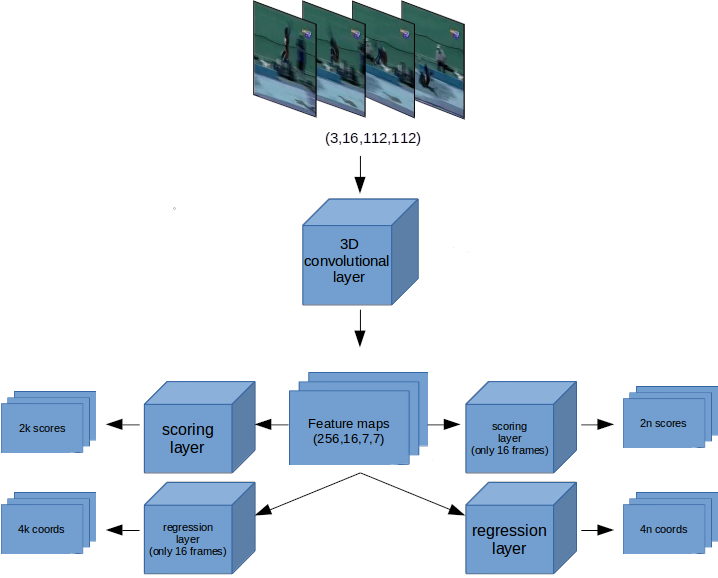
\includegraphics[scale=0.5]{tpn_1_2}
  \caption{TPN structure after adding 2 new layers, where k = 5n.}
  \label{fig:tpn_1_2}
\end{figure}

Training and Validation procedures remain the same. The only big difference is that now we have from 2 difference system proposed TOIs. So, we first concate
them and, then, we follow the same procedure. For training loss, we have 2 different cross-entropy losses and 2 different smooth-L1 losses, each for every
layer correspondly. The regressor does not change at all.

\subsection{Changing Regressor}
As the above results show, when we translate a TOI into a sequence of ROIs, recall reduces about 20-30\%. As a result, we should find a solution, in order to
deal with this proble.
\paragraph{From 3D to 2d}
The first idea we thought, was to change the first Convolutional layer from 3D to 2D. This means that we consider  features  not to have temporal dependencies for
each fra. As we can see in the figure \ref{}, we got worse results, so, we rejected this idea.
\paragraph{Remove time-mean layer}
The second idea was to remove the mean layer in time dimension. This means that, the input of the first linear layer after the 3D convolutional layer gets as
input all the features outputed from 3D convolution. 
\paragraph{Use max pooling instead of mean layer}


\par
As we noticed from the above figures, our system has difficulty in translating 3D boxes into 2D sequence of ROIs. So, that makes us rethink the way we designed
our TPN.
\subsection{Changing training procedure}
Until now, we trained TPN and regressor together, using one total loss, which was the sum of all the sublosses. Now we use a new approach.
At first, we  train TPN for 40 epochs. Then, we freeze TPN and we train the regressor for 20 epochs.


\section{ 3D anchors as 4k-dim vector}
In this approach, we set 3D anchors as 4k coordinates (k = 16 frames = sample duration). So a typical anchor is written as ($x_1, y_1, x'_1, y'_1, x_2, y_2, ...$)
where $x_1, y_1, x'_1, y'_1 $ are the coordinates for the 1st frame, $x_2, y_2, x'_2, y'_2$ are the coordinates for the 2nd frame etc as presented in \cite{DBLP:journals/corr/abs-1712-09184}.
In figure \ref{fig:anchor_4k} we can an example of this type of anchor.

\begin{figure}[h]
  \centering
  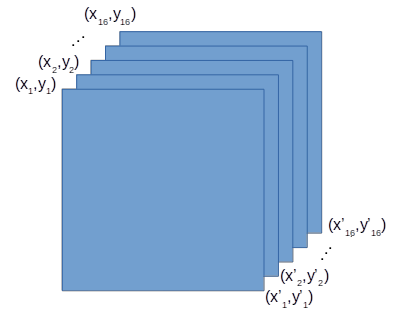
\includegraphics[scale=0.5]{anchor_4k}
  \caption{An example of the anchor $(x_1,y_1,x'_1,y'_1,x_2,y_2, ...)$}
  \label{fig:anchor_4k}
\end{figure}

The main advantage of this approach is that we don't need to translate the 3D anchors into 2D boxes. However, it has a big drawback, which is the fact that this type of anchors
has fixed time duration. In order to deal with this problem, we set anchors with different time durations, which are 16, 12, 8 and 4. Anchors with duration $ < $
sample duration (16 frames) can be written as 4k vector with zeroed coordinateds in the frames bigger that the time duration. For example, an anchor with
2 frames duration, starting from the 2nd frame and ending at the 3rd can be written as (0, 0, 0, 0, $x_1, y_1, x'_1, y'_1, x_2, y_2, x'_2, y'_2$, 0, 0, 0, 0) if sample
duration is 4 frames. 

\begin{figure}[h]
  \centering
  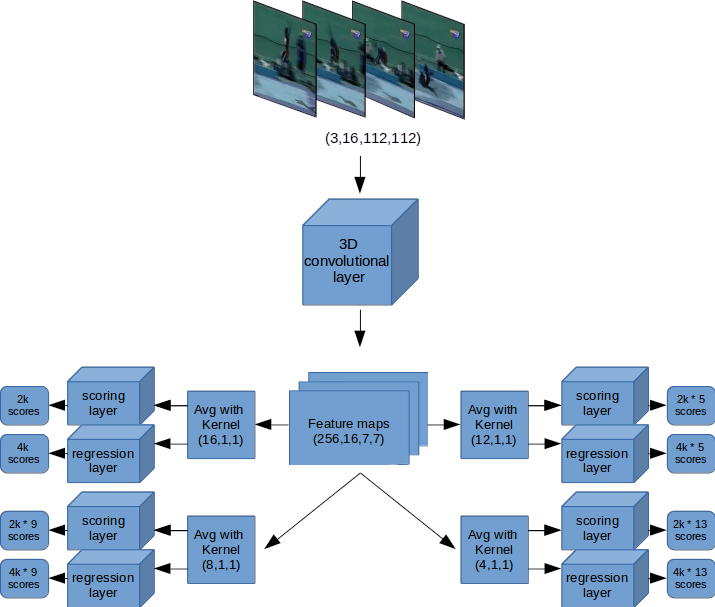
\includegraphics[width=1.\textwidth]{tpn_2}
  \caption{The structure of TPN according to new approach}
  \label{fig:New_structure}
\end{figure}

This new approach led us to change the structure of TPN. The new one can is presented in figure \ref{fig:New_structure}. As we can see, we \
added scoring and regression layers for each duration.

\subsection{Training}
In following figures we can see recall performance for sample duration = 16 when using max or avg pooling. 
% \begin{center}
%   % \begin{tabu} to 0.8\textwidth { | X[l] | X[c] | X[r] | }
%   \begin{tabular} { | c | c | c | c |}
%     \hline
%     \textbf{Duration} & \textbf{Type of Pooling} & \textbf{Dataset}  &  \textbf{Threshold } & \textbf{recall}\\
%     \hline
%     16  & Avg  & jHMDB  &  0.5 & \\
%     \hline
%     % \end{tabu}
%   \end{tabular}
% \end{center}
From the above results, we can see that using max pooling achieves better results.

\subsection{Adding regressor}
In full correspondance with the previous approach, we added an regressor for trying to find better results. We 
TODO
\subsection{Trying to  improve performance}
TODO
\subsection{Changing training procedure}
TODO
\subsection{Changing sample duration}
After trying all the previous version, we noticed that we get about the same recall performances. So, we thought that we could try
to reduce the sample duration. On top of that, we trained our network for sample duration = 8 and 4 frames.

.......................


\end{document}

